%\chaptermark{}ter{Finding low--energy spectrum of spin glass using CUDA}
\chapter[Brute--forcing spin--glass problems]{Brute--forcing spin--glass problems with CUDA}
\label{chapter:bruteforce}
In chapter \ref{chapter:tn} we presented a tensor network--based heuristic algorithm specifically
tailored for Ising spin--glass problems defined on Chimera graphs. In stark contrast, in this
chapter we will shift our attention to a deterministic algorithm capable of solving problems defined
on arbitrary (but relatively small) graphs.

Conceptually, the simplest approach for solving any optimization problem is a
brute force approach, i.e. an exhaustive search through the set of all possible
solutions. For the QUBO or Ising spin--glass with $N$ variables, this would
require iterating over $2^{N}$ possible states and computing energy for each of
them, resulting in a superexponential algorithm. Although the approach is
clearly infeasible for large problems, it presents several advantages. The
algorithm is deterministic and can certify\footnote{i.e., prove that the found
  solution is in fact optimal} the solution. Moreover, it can be used to compute
a low energy spectrum of arbitrary size $k$ (provided that it can fit into
memory). Lastly, it is trivially parallelizable and hence can be efficiently
accelerated using virtually any parallel computing paradigm, thus significantly
increasing attainable problem sizes.

In this chapter, we discuss such a brute--force algorithm using massively
parallel CUDA architecture. We start by outlining the basic version of the
algorithm and then discuss its recent optimizations for cases when the goal is
to find only the ground state (as opposed to finding a low energy spectrum).
Our implementation is capable of finding the ground state of instances of size
$N=50$ in an hour using a commodity GPU and achieving the same task in less
than 5 minutes on a server--grade NVIDIA DGX H100. Lastly, we present a
possible application of our algorithm, which is validating a recent MPS--based
algorithm for solving Ising spin--glasses.

% Optimization problems play an important role in modern society, especially in current volatile times. Instances of such problems can be found in numerous areas of industry and applied sciences. One could mention logistic issues, such as vehicle routing problem together with its variants, and the famous protein folding problem or job shop scheduling to name just a few. It is often the case where many of the aforementioned problems fall into the so called NP--hard complexity class. This fact alone renders hard to solve, making the entire operational research a challenging endeavour requiring enormous amount of computational resources.

% One way to tackle optimization problems is an exhaustive search over all possible solutions. Unfortunately, such brute--force approach quickly becomes impractical, as the number of possible solutions increases exponentially with the problem size. Nevertheless, despite its simplicity and obvious limitations, the brute--force algorithm is often the only approach capable of solving and certifying~\footnote{(i.e., proving that the found solution is in fact optimal)} \textit{arbitrary} problem instances within a given complexity class. For this very reason, efficient brute--force solvers are still considered to be an irreplaceable tool for testing and benchmarking other, often way more sophisticated, algorithms.

\section{Finding low--energy spectrum with CUDA}
\subsection{Outline of the algorithm}
An idealized brute force algorithm for solving QUBO problems running on a
hardware with infinite storage and an infinite number of execution units can be
summarized as follows:
\begin{enumerate}
  \item Launch number of threads equal to the total number of possible states.
  \item Let each thread compute the energy of one of the states.
  \item Extract (e.g. by sorting) the desired number of low--energy states.
\end{enumerate}
Naturally, an attempt to implement such an algorithm on real hardware is doomed
to fail. To exemplify this, consider a problem with $N=40$ variables. Assuming
we use 32-bit floating point numbers, one would need an enormous amount of
$2^{40}\cdot 4B = 4398046511104\mbox{B}$, or $4\mbox{TB}$ of working memory to
store the computed energies. For $N=50$, this number grows to $4096\mbox{TB}$.
Clearly, such an amount of needed memory is prohibitively large, and that is
even before we consider some form of storage for system states. Moreover, no
current hardware can execute $2^{40}$ threads in parallel. Fortunately, we can
adapt our algorithm to take into account limited memory and parallelism. To do
so, we introduce the following assumptions:
\begin{enumerate}
  \item We will process the solution space in \emph{chunks} that can fit into GPU
    memory.
  \item Number of states in a chunk can be larger than the total number of threads.
    Should this be the case, the threads will process the chunk using a
    grid--stride loop pattern.
\end{enumerate}
As an added benefit of our assumptions, we decouple the grid size from the
problem size. The number of thread blocks and block size become parameters of
our algorithm, which facilitates further fine-tuning of kernel execution
parameters.

The algorithm will keep track of $k$ lowest--energy states computed so far.

This information will be updated after each new chunk is processed. The
downside of this approach is that the size of the low--energy spectrum we can
compute is limited by the chunk size. However, this limitation is not as severe
as it seems, because in a typical scenario, we have $k \ll 2^{N}$.

In the next section, we discuss another important aspect of our algorithm,
which is efficient storage and representation of system states.

\subsection{Storage and representation of system states}
Implementing efficient algorithms involves choosing the right storage strategy
for the data the algorithm operates on. This is especially the case for
present-day GPUs, which are equipped with fairly limited memory, as compared to
the operating memory available to the traditional CPU. Moreover, memory
transfers between host and GPU induce additional overhead that should be
avoided whenever possible. For this reasons one often aims for designing the
storage strategy such that it reuses information already available on the GPU
as much as possible, thus optimizing resource usage and minimizing the number
of memory transfers.

In principle, each configuration of a $N$--variable QUBO can be represented by
$N$ integers. However, since each variable can be assigned only one of two
possible values, this wastes a lot of available memory, as out of each machine
word only a single bit is used. Instead, one can pack the whole state of the
system into a single integer by identifying each bit of the underlying machine
word with a single spin. In our implementation, we decided to use 64-bit
integers. This particular implementation choice limits attainable problem sizes
to $N=64$. However, considering that solving larger problems using the brute
force approach is not likely to be possible in the near future (as demonstrated
by our benchmarks presented further in this chapter), this is not a significant
limitation. Furthermore, should the need arise, one could extend the
implementation to use multiple 64-bit integers for storing a single
configuration.

Identifying states with integers greatly simplifies their enumeration, as it
boils down to iterating over an appropriate range of natural numbers. More
importantly, it allows GPU threads to identify the system state they have to
process using their index and additional offset designating the chunk. In our
implementation, we restrict ourselves to chunk sizes being power of two, i.e.
chunk size $=2^{M}$ for some $M < N$. We conceptually split each configuration
into two parts:
\begin{enumerate}
  \item A \emph{local} part comprising least significant $M$ bits. This is part is
    \emph{different} for each state in the chunk.
  \item A \emph{suffix} comprising the most significant $N-M$ bits. This part is
    \emph{the same} for each state in the chunk.
\end{enumerate}
Now, since there are $2^{N-M}$ chunks, we can identify each chunk with a $N-M$
bit number. Finally we arrive for a formula for an integer representation
$\mathbf{q}_{i}^{j}$ of an $i$-th configuration in $j$-th chunk:
\begin{equation}
  \mathbf{q}_{i}^{j} = i + 2^{M}\cdot j,\qquad i=0,\ldots,2^{M}-1, \; j=0,\ldots,2^{N-M}-1
\end{equation}
The following example demonstrates the representation described above in
detail.
\begin{example}[Processing solution space in chunks]
  Consider QUBO with $N=8$ variables. We decide to use $M=5$. Hence, there are
  $2^{M}=32$ states in each chunk and a total of $2^{N-M}=8$ chunks. The
  \emph{local} part of the first state in each chunk is $0$, or $(00000000)_{2}$
  in binary. The local part of the last state in each chunk is $31$, or
  $(00011111)_{2}$. The table \ref{tab:chunks} below enumerates ranges of
  combined integer representation of states in each chunk.
  \begin{table}[ht!]
    \centering
    \begin{tabular}{|c|c|c|c|c|c|}
      \hline
      \rowcolor{theader}
      \multicolumn{2}{|c|}{Chunk}       &
      \multicolumn{2}{c|}{First state} &
      \multicolumn{2}{c|}{Last state}                                                                         \\
      \hline
      \rowcolor{tsubheader} Index                            &  Binary    & Decimal & Binary           & Decimal & Binary           \\
      \hline
      0                                & $(000)_2$ & 0       & $(00000000)_{2}$ & 31      & $(00011111)_{2}$ \\
      1                                & $(001)_2$ & 32      & $(00100000)_{2}$ & 63      & $(00111111)_{2}$ \\
      2                                & $(010)_2$ & 64      & $(01000000)_{2}$ & 95      & $(01011111)_{2}$ \\
      3                                & $(011)_2$ & 96      & $(01100000)_{2}$ & 127     & $(01111111)_{2}$ \\
      4                                & $(100)_2$ & 128     & $(10000000)_{2}$ & 159     & $(10011111)_{2}$ \\
      5                                & $(101)_2$ & 160     & $(10100000)_{2}$ & 191     & $(10111111)_{2}$ \\
      6                                & $(110)_2$ & 192     & $(11000000)_{2}$ & 223     & $(11011111)_{2}$ \\
      7                                & $(111)_2$ & 224     & $(11100000)_{2}$ & 255     & $(11111111)_{2}$ \\
      \hline
    \end{tabular}
    \caption{An example enumeration of chunks iterated over by brute force algorithm.}
    \label{tab:chunks}
  \end{table}

  \begin{table}{}

  \end{table}
\end{example}

\subsection{Performance benchmarks}

\subsection{Implementation details}

In our approach we decided to store states and their corresponding energies in
arrays of size $k+2^{M}$, where $k$ is the desired size of the low energy
spectrum and $2^{M}$ is the chunk size. The arrays are always synchronized,
i.e. at all times $i$-th state corresponds to $i$-th energy. The first $k$
elements store the lowest energies and corresponding configurations found so
far. When a new chunk is being processed, the second part of the arrays is
populated with new states and energies by the energy--computing kernel. Next,
the best $k$ states from the current chunk are selected and moved into indices
$k, k+1,\ldots,2k-1$. In this way, the global best solutions from previous
chunks and the lowest energy states from the current chunk in a continuous
space in memory, which facilitates updating the best configurations.

One could use a parallel sorting procedure for extracting the $k$
lowest--energy states at each step. However, for improved performance, we
decided to use a combination of the \texttt{bucketSelect} \cite{bucketselect}
algorithm in tandem with \texttt{thrust::partition\_by\_key} \cite{thrust}. The
\texttt{bucketSelect} algorithm is used to find the pivot configuration that
would reside at $k$--th position in the sorted array. Then,
\texttt{thrust::partition\_by\_key} is used to reorder both arrays such that
the configurations with energies lower than the one of the pivot are moved to
the beginning. The same procedure is used both for extracting the $k$-lowest
energy states in the given chunk, as well as to update the global solution by
extracting $k$-lowest energy configurations from the first $2k$ configurations.
The whole procedure is depicted in Fig. \ref{fig:bruteforce}.

Lastly, we would like to note that the algorithm we just described can also be
implemented on homogenous, CPU--only architectures using any of the available
parallelization approaches. In our implementation, we used the
OpenMP\cite{openmp} for a CPU--only version.

\begin{figure}
  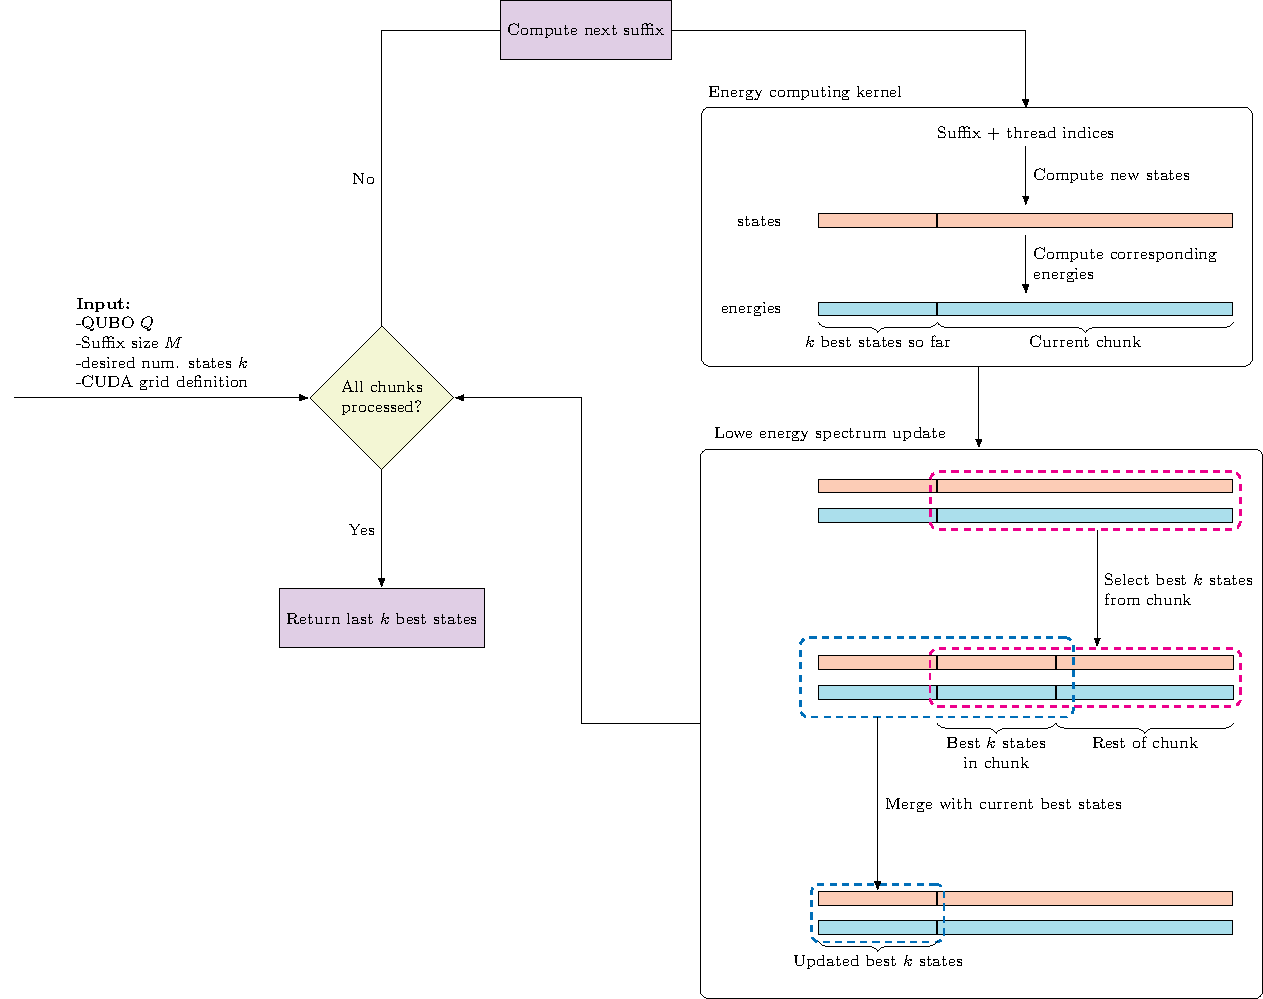
\includegraphics[width=\textwidth]{figures/bruteforce}
  \caption{
    Detailed representation of brute force algorithm for finding $k$-lowest energy
    states of a QUBO. The algorithm iterates over the set of all possbile states in
    chunks of size $2^{M}$, where $M$ is a user--defined parameter. Throughout the
    algorithm execution, we maintain arrays of states and corresponding energies.
    The first part of those arrays stores the $k$ best configurations encountered
    so far, and the second part stores configurations belonging to the currently
    processed chunk. In the first phase of the iteration, an energy--computing
    kernel is launched. Then, the $k$--lowest energy configurations from the given
    chunk are selected and moved towards the part of the array with the current
    best solutions. Finally, the best $k$ states are selected from the first $2k$
    configurations and the algorithm proceeds to the next chunk, or terminates if
    all the chunks have been iterated over. } \label{fig:bruteforce}
\end{figure}

\subsection{Performance benchmarks}
In order to test the performance of our algorithm, we run extensive benchmarks
using the following hardware:
%
\begin{itemize}
  \item CPU:
    \href{https://ark.intel.com/products/94456/Intel-Core-i7-6950X-Processor-Extreme-Edition-25M-Cache-up-to-3-50-GHz-}{$10$
      Cores {\rmfamily Intel\textregistered} Core \textsuperscript{TM}i7-6950X};
    %
  \item GPU(1):
    \href{https://www.nvidia.com/en-us/geforce/products/10series/geforce-gtx-1080}{Nvidia
      GeForce GTX $1080$, $8$GB GDDR$5$ global memory, $2560$ CUDA Cores};
    %
  \item  GPU(2): \href{https://www.nvidia.com/en-us/titan/titan-v/}{Nvidia Titan V,
      $12$GB HBM$2$ global memory, $5120$ CUDA Cores}.
\end{itemize}

For conducting our benchmarks we generated $100$ spinglass instances for each
$N=24, 26, \ldots, 30, 32$. Additionally we generated $100$ instances of size
$N=40$ and single instances of sizes $N=48, 50$ that were feasible to solve
with Titan V GPU. Coefficients of each spinglass were drawn randomly from
uniform distributions on the intervals $[-2, 2]$ and $[-1, 1]$ for magnetic
fields and couplings respectively. For each instance, we computed low energy
spectrum of $k=100$ states with our algorithm. We used maximum chunk size of
$2^{29}$ for Titan V and CPU and chunk size of $2^{27}$ for GTX 1080.

As already mentioned, larger instances $(N > 32)$ were solved only using Titan
V GPU. For GTX 1080 and CPU implementation, the expected time to solve those
instances was estimated based on the timings for smaller $N$. The results of
our benchmarks are are presented in Fig. \ref{fig:benchmark_results}.

\begin{figure}
  \centering
  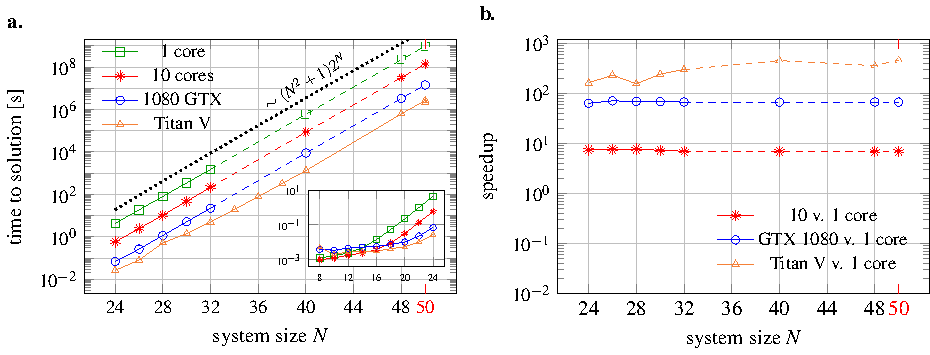
\includegraphics[width=\textwidth]{figures/resultsplot_reduced.pdf}
  \caption{Results of benchmarks of our algorithm. {\textbf{a.}} Time to solution vs.
    system size $N$. {\textbf{b.}} Speedup of multi-core/GPU implementation with
    respect to a single core one vs. system size $N$. The solid lines represent the
    numerical results and the dashed lines present estimates based on results
    obtained for smaller system sizes.} \label{fig:benchmark_results}
\end{figure}

\section{Improving the algorithm using Gray Code}

The algorithm presented in the previous chapter and its GPU--enabled
implementation are already highly performant. However, we can still improve
upon it by altering the order in which we enumerate the integral representation
of states used by our algorithm.

\subsection{Single bit--energy difference}
Suppose we are given a QUBO with $F(q_{1},\ldots,q_{N})$ as in the equation
\ref{eq:qubo}. Consider two states, say $\bq{1} = (\q{1}_{1},\ldots,\q{1}_{N})$
and $\bq{2}=(\q{2}_{1},\ldots,\q{2}_{N})$ such that they only differ in the
$k$-th bit, i.e. $\q{2}_{k}=1-\q{1}_{k}$ and $\q{2}_{i}=\q{1}_{i}$ for $i \ne
  k$. The energy difference $F(\bq{2})-F(\bq{1})$ can be easily computed and the
formula reads
\begin{align}
  \begin{split}
    \label{eq:energydiff1}
    F(\bq{2})-F(\bq{1}) &= b_{k}(\q{2}_{k}-\q{1}_{k}) + \sum_{i\ne k}a_{ik}\q{1}_{i}(\q{2}_{k} - \q{1}_{k}) \\
    &= (\q{2}_{k}-\q{1}_{k}) \left(b_{1} + \sum_{i \ne k}a_{ik}\q{1}_{i}\right) \\
    & = (1-2\q{1}_{k}) \left(b_{k} + \sum_{i \ne k}a_{ik}\q{1}_{i}\right).
  \end{split}
\end{align}
Interestingly, computing the difference in equation \eqref{eq:energydiff1}
requires only $N$ multiplications. But how can this be used to improve the
performance of the exhaustive search through QUBO state space?

Moving $F(\bq{1})$ to the right-hand side, we obtain a formula for $F(\bq{2})$,
which allows for computing it with only $N+1$ instead of maximum of $N(N+1)/2$
multiplications, provided that $F(\bq{1})$ is known. Remember that this is only
possible because $\bq{1}$ and $\bq{2}$ differ only by a single bit. If we could
enumerate states in such a fashion that every consecutive two states differ
only by a single bit, we could leverage the above formula instead of
recomputing energy for each state from scratch. Before we describe how the
procedure works and how to implement this on GPU, let us first introduce the
necessary notation. Given a state $\mathbf{q} = (q_{1},\ldots,q_{N})$, by
$\flip{\mathbf{q}}{k}$ we will denote a state resulting from flipping $k$-th
bit of $\mathbf{q}$, i.e.
\begin{equation}
  \flip{\mathbf{q}}{k} \coloneq (q_{1}, \ldots, q_{k-1}, 1-q_{k}, q_{k+1}, \ldots, q_{N})
\end{equation}
and by $\diff_{F}(\mathbf{q},k)$ we will denote the difference between the
energies of $\flip{\mathbf{q}}{k}$ and $\mathbf{q}$. Using the equation
\eqref{eq:energydiff1}, we see that the expression for
$\diff_{F}(\mathbf{q},k)$ is
\begin{align}
  \begin{split}
    \diff_{F}(\mathbf{q},k) = F(\flip{\mathbf{q}}{k}) - F(\mathbf{q}).
  \end{split}
\end{align}
The pseudocode for a serial algorithm for solving a QUBO problem using our
observations is outlined in listing \ref{lst:grayserial}. Before we can
implement it on GPU though, we need to answer the following questions:
\begin{lstlisting}[
  language=Python,
  caption={Pseudocode for algorithm solving the QUBO problem using energy differences and bit flips.},
  captionpos=b,
  label=lst:grayserial,
  float,
  floatplacement=H
]
def solve_qubo(F, q):
    q = [0] * N # Start with all bits set to 0
    best_state = current_state = q
    best_energy = current_energy = F(q)

    for i in range(2 ** N - 1):
        k = find_next_bit_to_flip(i)
        current_energy = current_energy + diff(q, k)
        current_state = flip(q, k)
        if current_energy < best_energy:
            best_energy = current_energy
            best_state = current_state
    return best_state, best_energy
\end{lstlisting}
\begin{enumerate}
  \item How to produce a sequence of $2^{N}-1$ bits such that executing them enumerates
   a rll possible states?
  \item How to divide work among CUDA threads?
\end{enumerate}
The answer to the first question is well--known and involves enumerating
integers using the Gray code, which we will describe now.

\subsection{Gray code}
When one talks about a binary encoding of integers, the first thing that comes
to mind is a usual positional base-2 system. This encoding certainly does not
fit our purpose. Indeed, suppose $N=3$ and we are currently processing state
corresponding to number $3$, whose representation in binary is $(011)_{2}$. The
next state, corresponding to $4$ is encoded by the string $(100)_{2}$, which
differs in all three bits.

Instead of using the positional system, we might utilize an encoding called
Gray code, or Reflected Binary Code (RBC), which is primarily used to improve
the robustness of electromechanical switches and in error correction protocols.
In this code, encoding of two successive integers always differs by at most one
bit, which makes it suitable for application in our algorithm.

The conceptual construction of Gray code is straightforward. For Gray Code of
length $1$ we have two binary strings: $0$ and $1$. To obtain all Gray codes
for a given length $N > 1$, we first construct an ordered list of codes of
length $N-1$ and call it $L$. Then, we reverse the list of codes, and call it
$H$, an operation called \emph{reflection}. Finally, we prepend $0$ to all
elements of $L$ and prepend $1$ to all elements of $H$. The concatenation of
$L$ and $H$ forms the $N$--bit Gray Code. The process is illustrated in Fig.
\ref{fig:gray} .One useful consequence of the construction is that the shorter
Gray Codes might be viewed as initial parts of the larger ones prepended with
enough zeros. Thus, statements as ``$n$-th Gray code'' make sense and are
unambiguous.

\begin{figure}
  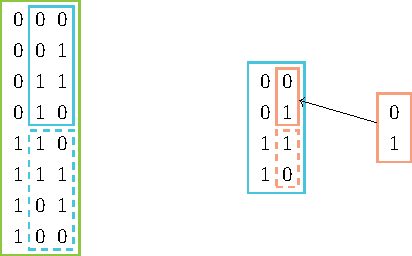
\includegraphics[width=\textwidth]{figures/gray.pdf}
  \caption{Reflection--based construction of Gray Code. The length of the code is denoted
    by $N$. For $N=1$, the code comprises two binary strings, $0$ and $1$. To
    construct the code of length $N>1$, the code of length $N-1$ and its vertical
    reflection are stacked. Then, the first, unreflected half is prepended with $0$
    while the second, reflected half is prepended with $1$.} \label{fig:gray}
\end{figure}

An important thing to observe is that in our algorithm we need at most two Gray
Code--encoded numbers at the time to determine the bit to be flipped. The
reflection--based construction outlined so far would require precomputing a
large part (if not all) of the encodings at once. Considering the size of the
state space, this is clearly infeasible. However, there exists an explicit
formula for computing $n$-th Gray code, which reads:
\begin{equation}
  \mbox{gray}(n) = n \oplus (n >> 1),
\end{equation}
where $\oplus$ denotes the bitwise xor operation and $>>$ is right bitshift.

To compute which bit differs between consecutive Gray codes, we can xor them,
and then find the position of the only set bit in the resulting integer. One
can easily implement a function that finds the first set bit in a 64-bit
integer, or use one of the available library or compiler-builtin functions. For
instance, POSIX--compatible C standard libraries include \texttt{ffsll}
function. In CUDA, there is a \texttt{\_\_ffsll} function available. For both
of the above cases, the function counts bits from $1$. Using this convention,
we can write a pseudocode for a function \texttt{find\_bit\_to\_flip} from
listing \ref{lst:grayserial} like in the listing \ref{lst:findbit}

\begin{lstlisting}[
  language=Python,
  caption={Pseudocode for a function generating bit flips for Gray code construction},
  captionpos=b,
  label=lst:findbit,
  float,
  floatplacement=H
]
def find_bit_to_flip(i): # i starts from 0
    return ffs(gray(i) ^ gray(i+1))
\end{lstlisting}

Now that we know how to construct a correct sequence of bit flips, it is time
we design parallelization strategy, which is what we will do next.

\subsection{Parallelization using GPU}
The algorithm presented in \ref{lst:gray} is fully serial. Our task is now to
parallelize it so that it can be executed on GPU. Unsurprisingly, we will once
again employ the strategy of dividing each state into a suffix and a prefix
part. This time, however, it is the suffix that will stay fixed between
iterations. The prefix part will be updated in each iteration by flipping a
single bit in Gray code order. The process is illustrated in Fig.
\ref{fig:grayparallel}.

\begin{figure}
  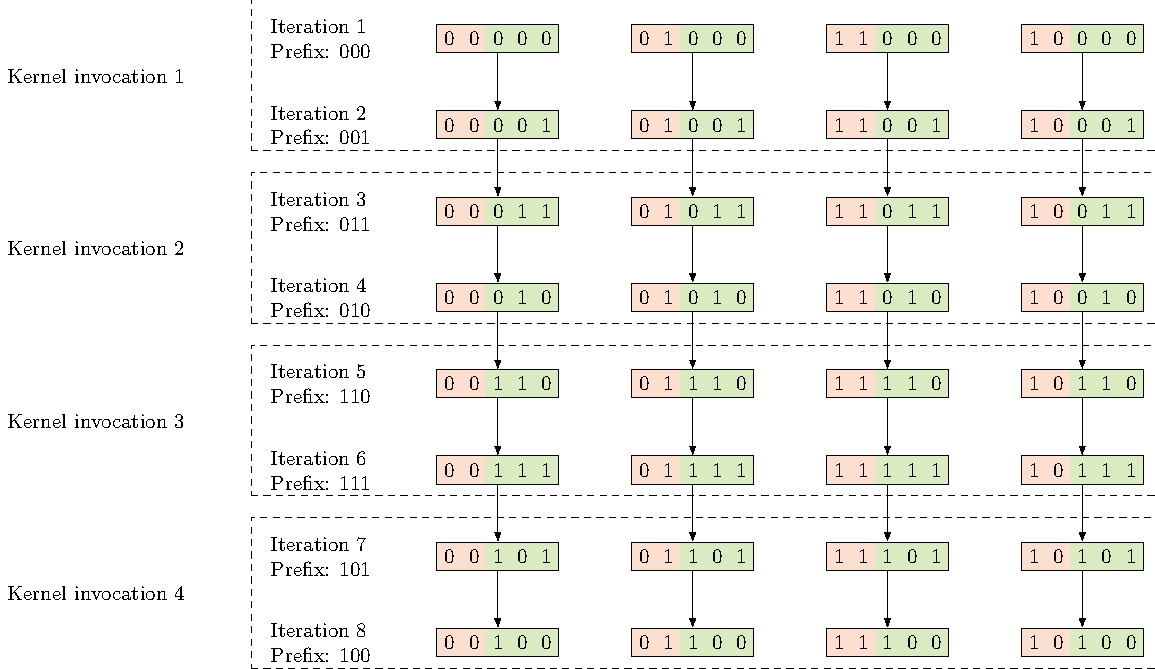
\includegraphics[width=\textwidth]{figures/grayparallel}
  \caption{
    Parallel processing of $N$--variable QUBO configurations in Gray code order. In
    our example, suffix length $M=2$, and hence $2^{M}=4$ states are processed in
    each iteration. Consequently, there are $2^{N-M}=8$ iterations. For this
    example, we consider a kernel that computes two iterations per kernel
    invocation, resulting in $2^{N-M}/2 = 4$ kernel invocations total. }
  \label{fig:grayparallel}
\end{figure}

Throughout the execution of the algorithm, we maintain four arrays of size
$2^{M}$. In each array, the $i$-th item always corresponds to the $i$-th
suffix. The \texttt{best\_states} and \texttt{best\_energies} arrays store the
best states found so far amongst states with $i$-th suffix. The
\texttt{current\_states} and \texttt{current\_energies} store configuration and
corresponding energy of current state being processed for $i$-th suffix. Each
iteration starts by determining the index of the next bit to be flipped. This
value is the same for all suffixes. Next, the algorithm computes energy
difference using the equation \ref{eq:energydiff1} and updates the
corresponding energy accordingly. After all $2^{N-M}$ iterations, the
\texttt{best\_states} and \texttt{best\_energies} arrays are used to extract
the ground state.

It is crucial to note that since we are only interested in finding the ground
state, we can group several iterations in one kernel invocation. In fact, it is
entirely possible to implement a kernel that runs all the iterations, which
would avoid kernel launch overhead. Moreover, such kernel could use
thread--local variables to store current state and energy instead of using
global arrays, which would further increase performance. However, as we will
see further in this chapter, we will propose further optimizations that would
require us to split the algorithm into several kernel invocations.

\subsection{Further optimizing parallel execution}

There are two optimizations we can make to further reduce the number of
operations performed in each iteration. Let us first notice, that the only bit
flips that can happen, do so in the prefix part. Going back to the equation
\eqref{eq:energydiff1}, we can rewrite the expression for $F(\bq{2})-F(\bq{1})$
into a sum of two parts:
\begin{align}
  F(\bq{2})-F(\bq{1}) = & (1-2\q{1}_{k}) \left(b_{k} + \sum_{i=0,i\ne k}^{N-M-1}a_{ik}\q{1}_{i}\right) + \label{eq:energydiff2} \\
                        & (1-2\q{1}_{k}) \left(b_{k} + \sum_{i=N-M}^{N-1}a_{ik}\q{1}_{i}\right)\label{eq:energydiff3}
\end{align}
Since the first summand \eqref{eq:energydiff2} is independent from the suffix,
which means that for each of the considered suffixes in any given iteration, it
has the same value. Since the states in the iteration are processed in parallel
by GPU threads, we have to either redo the same computation multiple times, or
use some synchronization mechanism, e.g. compute the prefix in one thread in
each block and then propagate the result to the whole block through shared
memory. However, there is a third approach. For each iteration, we compute the
prefix part of the energy difference using CPU, and then use it as a kernel
parameter. More precisely, we compute $L$ values of the prefix part of the
energy difference and pass it to the kernel as an additional array. Since the
information about which bit to flip is also relevant, we pass the bit sequence
as another array as well.

As for the \eqref{eq:energydiff3} part, observe that for each given prefix
there are only $N-M$ possible values of $k$ (again, that's because the bit
flips happen only in the prefix part, and there are $N-M$ prefix bits).
However, not all values of $k$ are equally common. Examining the Gray code
construction (c.f. Fig. \ref{fig:gray}) reveals that the least significant bit
flips half of times and the second least significant bit flips a quarter of
times. Generally, for $k=0,\ldots,N-M-1$ the $k$-th bit flips constitutes
approximately \footnote{Approximately, because there is an odd number of
  $2^{N-M}$ -1 flips performed, because we do not perform last bit flip which
  would take us back to $(0,\ldots,0)_2$ prefix.} $1/2^{k+1}$ of times.
Therefore, we can cache the value of \eqref{eq:energydiff3} for the $K$ most
commonly--occuring bit flips, where $K$ is a user--controlled parameter.

\begin{figure}
  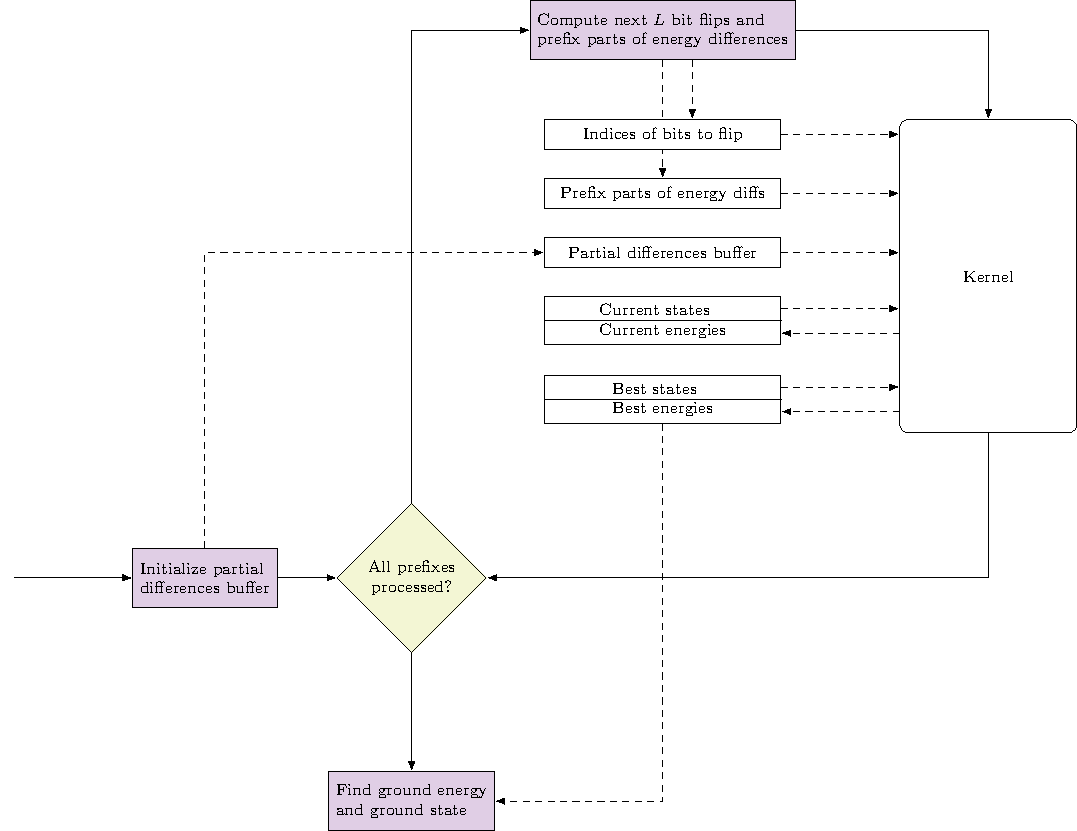
\includegraphics[width=\textwidth]{figures/bruteforcegray}
  \caption{
    Schematic representation of the GPU--enabled brute force algorithm for finding
    ground state of a QUBO problem using Gray codes.
  }
  \label{fig:bruteforcegray}
\end{figure}

\begin{figure}
  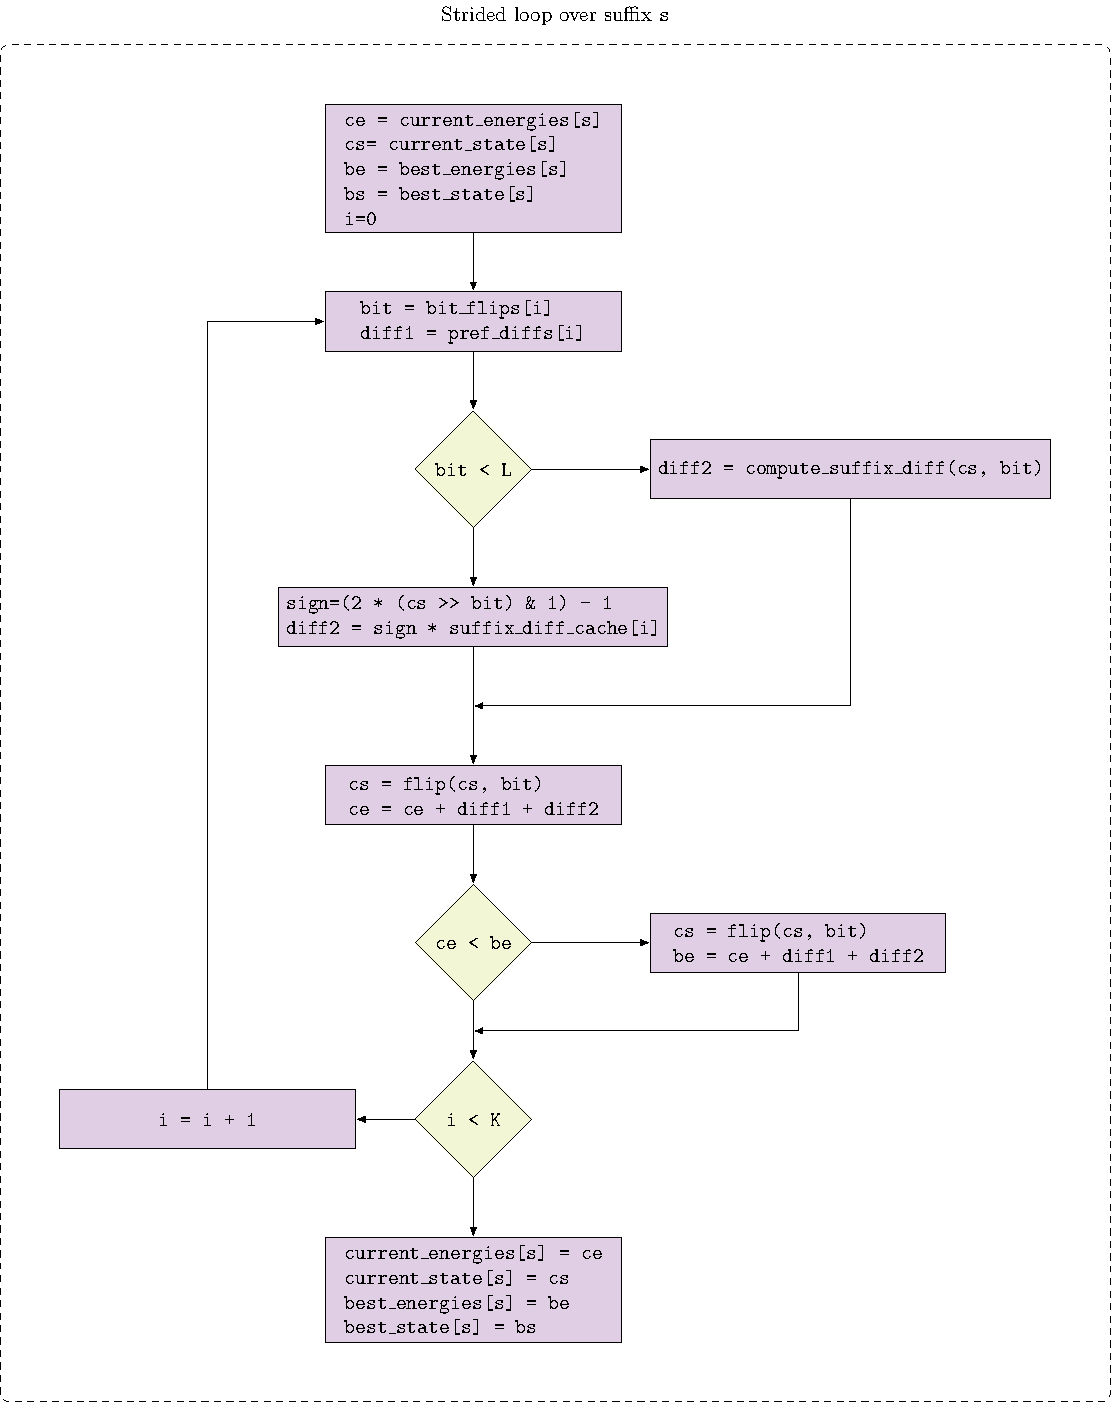
\includegraphics[width=\textwidth]{figures/bruteforcegray2}
  \caption{Implementation of the strided loop for kernel in fig \ref{fig:bruteforcegray}.}
\end{figure}

\subsection{Benchmarks}

\begin{figure}
  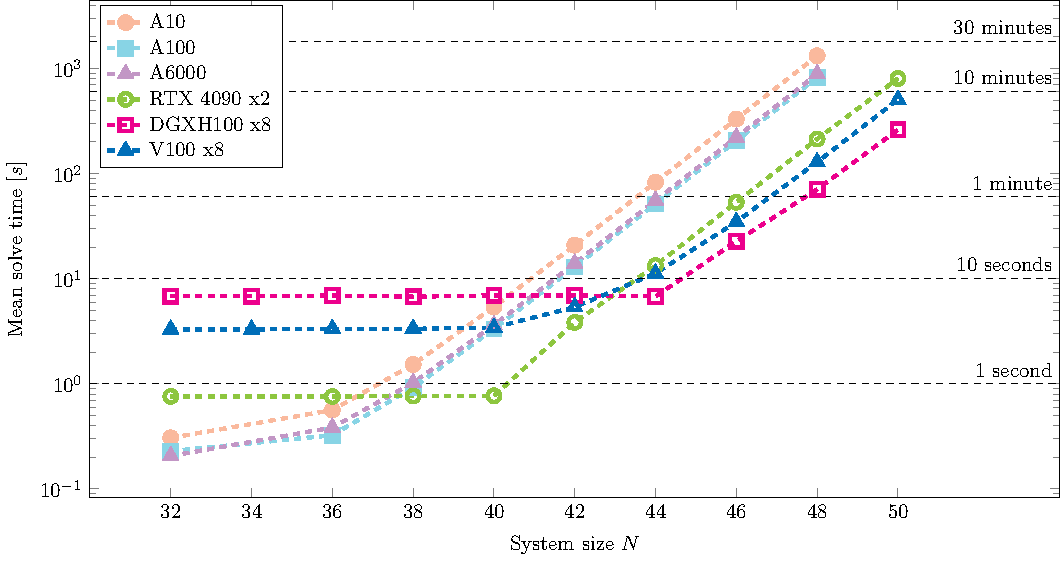
\includegraphics[width=\textwidth]{figures/bf_benchmarks_initial}
  \caption{
    Benchmarking results for Gray code--based brute force algorithm for finding a ground state
    of Ising model. The dashed lines between data points are provided for visual guidance. For each
    system size $N$, the solution times were averaged over 20 different instances with known ground
    states. Observe that for setups with multiple GPUs and small system sizes, the solution time
    remains virtually constant. This is because, for small system sizes, the execution time is
    dominated by tasks related to distributing work and gathering results. The parameters used for
    benchmarking in each setup are summarized in table \ref{tab:bruteforce-gs-only-table}.
  }
  \label{fig:bruteforce-gsonly-benchmarks}
\end{figure}

\begin{table}[!ht]
  \tiny
  \begin{tabular}{|l|c|c|c|c|c|}
    \hline
    \multirow{2}{*}{GPU(s)} & \multicolumn{2}{c|}{Kernel launch parameters} & \multicolumn{2}{c|}{Algorithm parameters} & \multirow{2}{*}{\makecell{\# Fixed \\ variables}}\\
    \cline{2-5}
     & Block size & Grid size & Suffix size & \makecell{\# Steps per \\ kernel launch} &\\
    \hline
    A10& 512 & 4096 & 27 & 4096 & N/A\\
    \hline
    A100& 512 & 4096 & 27 & 4096 & N/A\\
    \hline
    A6000 & 1024 & 4096 & 27 & 4096 & N/A\\
    \hline
    V100 x8 & 1024 & 4096 & 27 & 4096 & 3\\
    \hline
    DGX H100 x8 & 1024 & 8192 & 29 & 8192 & 3\\
    \hline
    RTX 4090 x8 & 512 & 4096 & 28 & 4096 & 1\\
    \hline
  \end{tabular}
  \caption{Parameters used for benchmarking}
  \label{tab:bruteforce-gs-only-table}
\end{table}
%%% Local Variables:
%%% mode: latex
%%% TeX-master: "../main"
%%% End:
